%--------------------------------------------------
\section{Proceso ajustado}


Con el desarrollo del sistema, un paciente, previamente registrado en el mismo, al presentar la necesidad de ser atendido por un médico, tendrá la opción de realizar una cita en línea donde el sistema le mostrará al paciente los horarios disponibles y no disponibles de cada día, separando cada horario para cada consultorio con su respectivo médico. Si el paciente agenda una cita en algunos de estos horarios disponibles, entonces una cita se generará para dicho horario y consultorio.\\ 

Hecho esto, el paciente debe de presentarse en la clínica 10 minutos antes de la hora de su cita para poder realizar el pago de la consulta con el cajero, para que el cajero pueda entonces realizar el registro de dicho pago y habilitar la cita.\\

Al ser atendido el paciente, el médico realiza el diagnóstico y tratamiento para la enfermedad del paciente en caso de existir dicha enfermedad, y el médico crea o actualiza el expediente del paciente con el diagnóstico y tratamiento.\\

Al finalizar la consulta, el paciente puede adquirir los medicamentos necesarios para el tratamiento en la farmacia de la clínica, donde el farmacéutico despacha los medicamentos, realiza el registro de la venta de medicamentos y el sistema actualiza el inventario de los mismos.\\

\subsection{Proceso de citas}
\begin{figure}[htbp!]
		\centering
			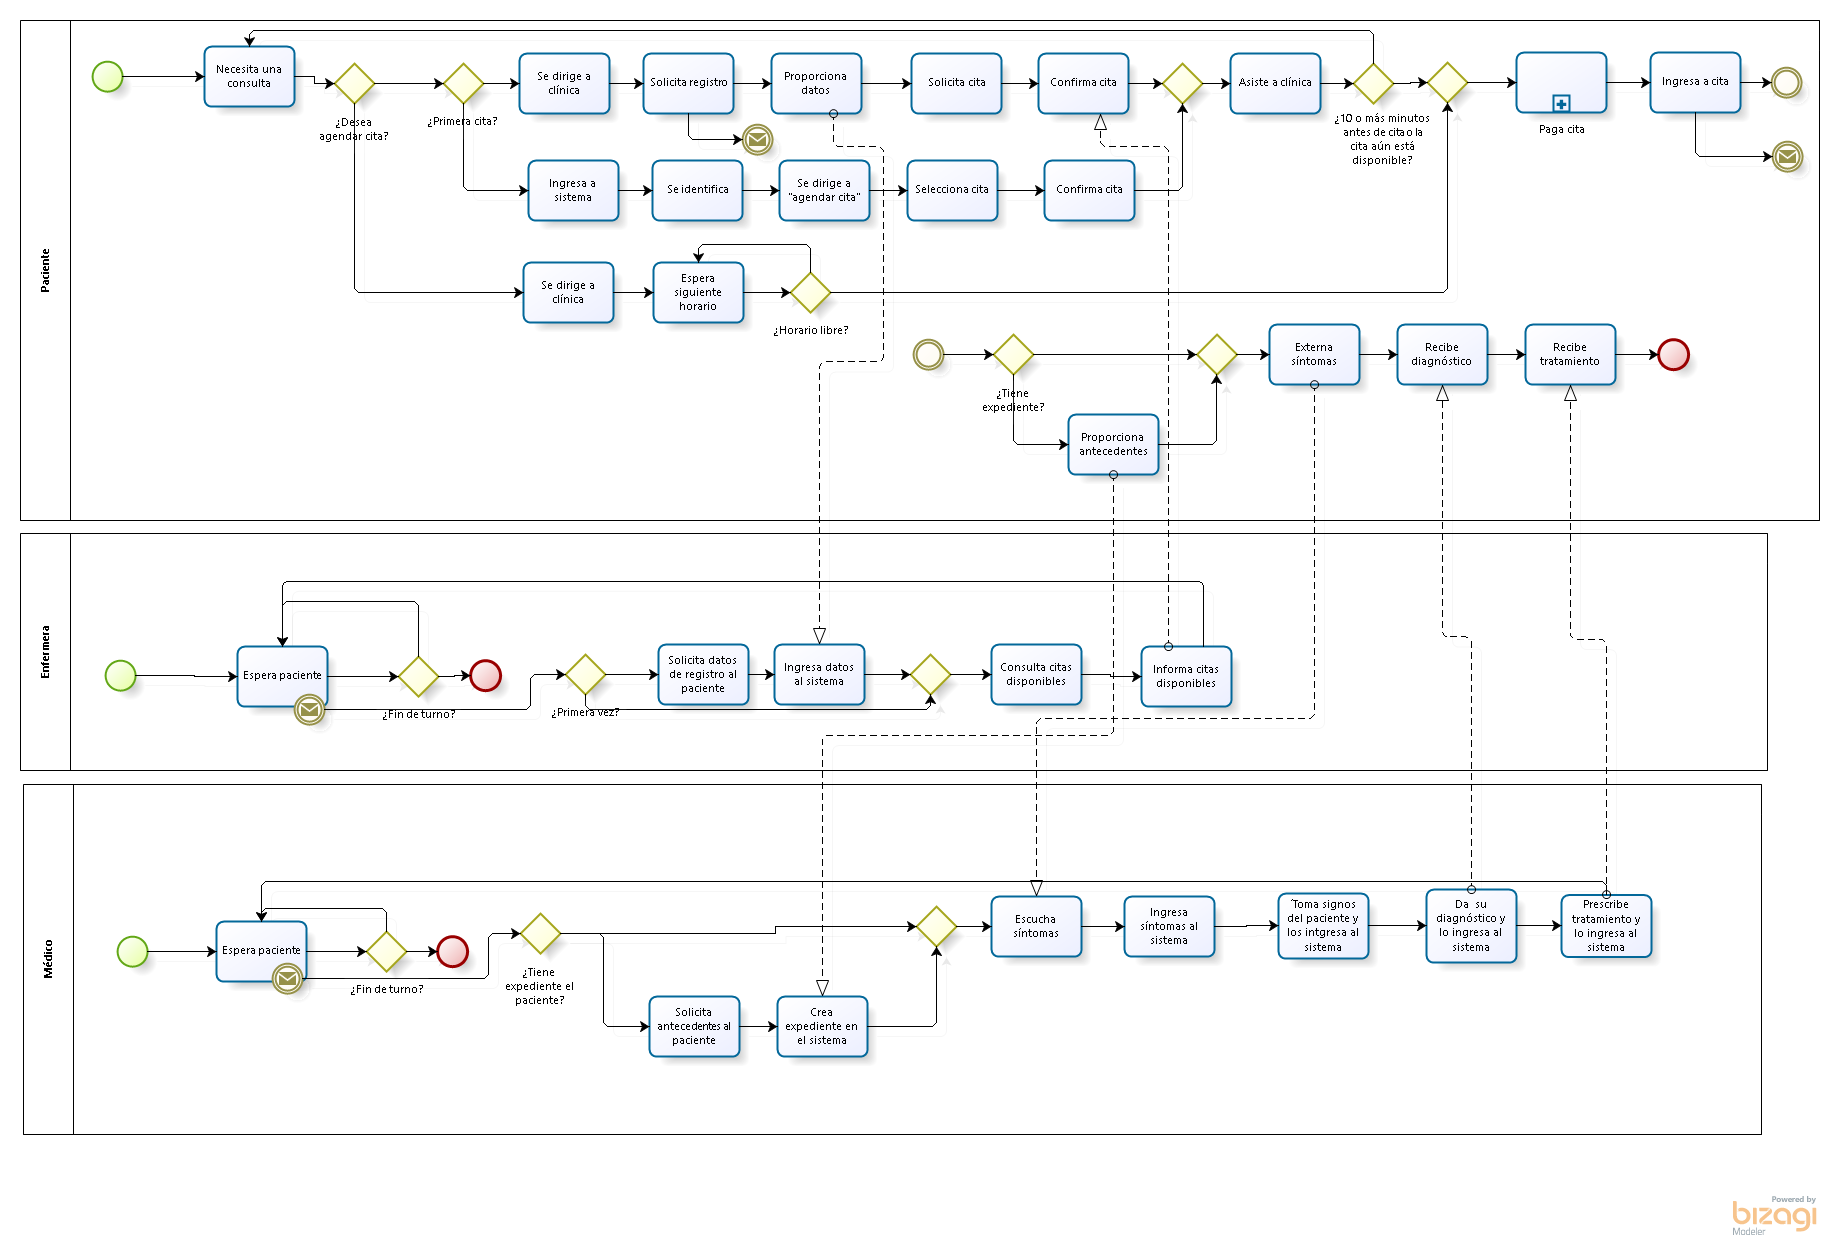
\includegraphics[width=1\textwidth]{images/Proceso_citas}
		\caption{Diagrama del proceso de citas.}
	\end{figure}
    
    \subsection{Proceso de pago de citas}
\begin{figure}[htbp!]
		\centering
			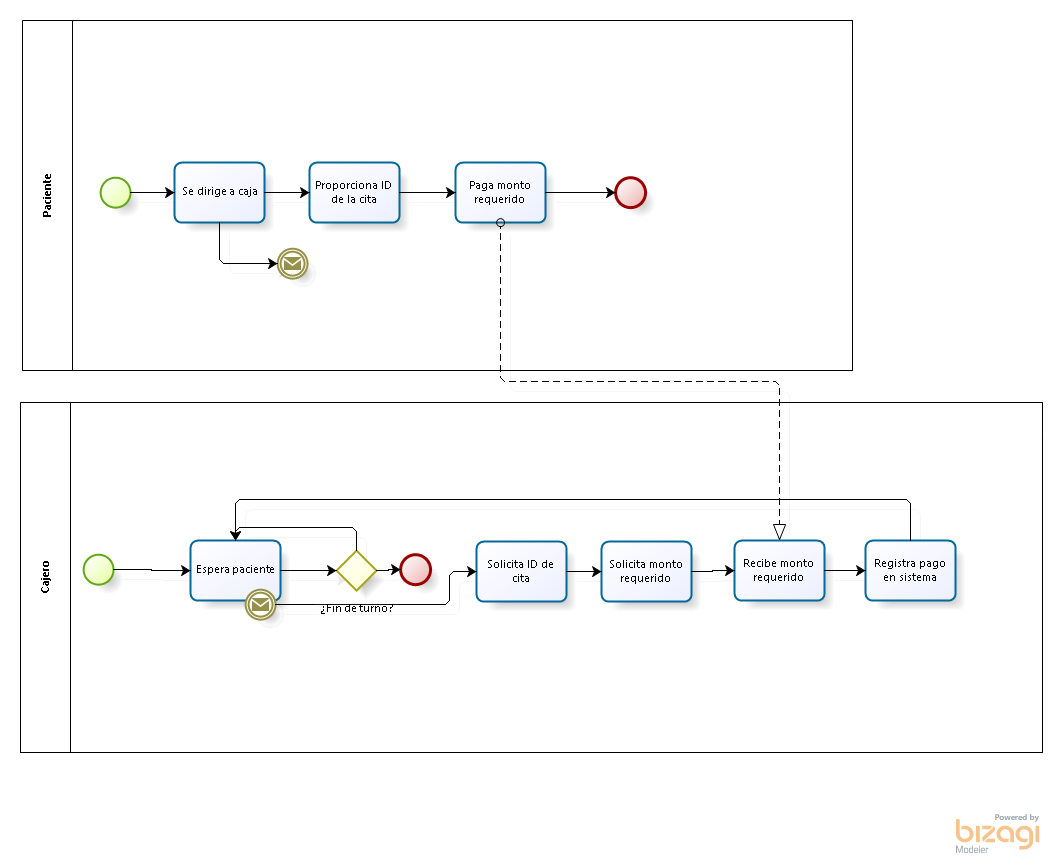
\includegraphics[width=0.7\textwidth]{images/Proceso_pago_cita}
		\caption{Diagrama del proceso de pago de citas.}
	\end{figure}
    
    \subsection{Proceso de adquisición de medicamentos}
\begin{figure}[htbp!]
		\centering
			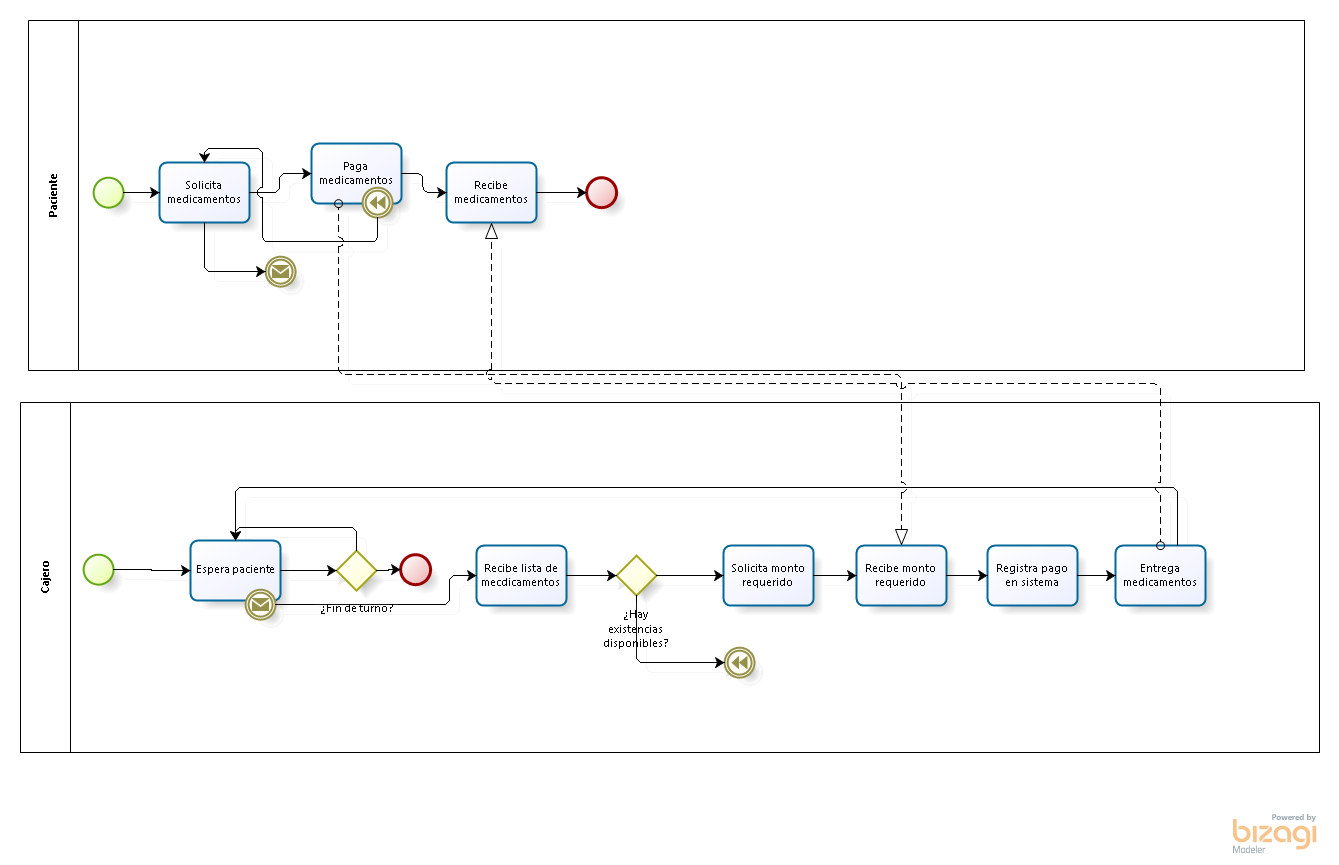
\includegraphics[width=0.7\textwidth]{images/Proceso_medicamentos}
		\caption{Diagrama del proceso de adquisición de medicamentos.}
	\end{figure}
\newpage
%--------------------------------------------------
\section{Procesos actuales}

% - - - - - - - - - - - - - - - - - - - - - - - - -
\subsection{Participantes}

\begin{itemize}
	\item \textbf{Paciente: }Es quien recibe los servicios médicos de la clínica. Debe asistir a la clínica o comunicarse vía telefónica para agendar una cita. Debe pagarla 10 minutos antes de su hora o podrá ser ocupada por otro paciente.
    \item \textbf{Enfermera: }Se encarga de la gestión de los horarios del consultorio. Es quien agenda las citas a los pacientes, y debe de proporcionar el expediente médico de los pacientes que se atenderán en el día al médico y si hay un paciente sin cita será la encargada de obtener su expediente.
    \item \textbf{Médico: }Es quien se encuentra dando servicio médico a los pacientes en un consultorio, debe de hacer modificaciones en el expediente cada que un paciente asista a una cita.
    \item \textbf{Cajero: }Se encarga de realizar cobros de citas y de la venta de medicamentos.
\end{itemize}
% - - - - - - - - - - - - - - - - - - - - - - - - -
\subsection{Proceso de citas}

\begin{figure}[htbp!]
		\centering
			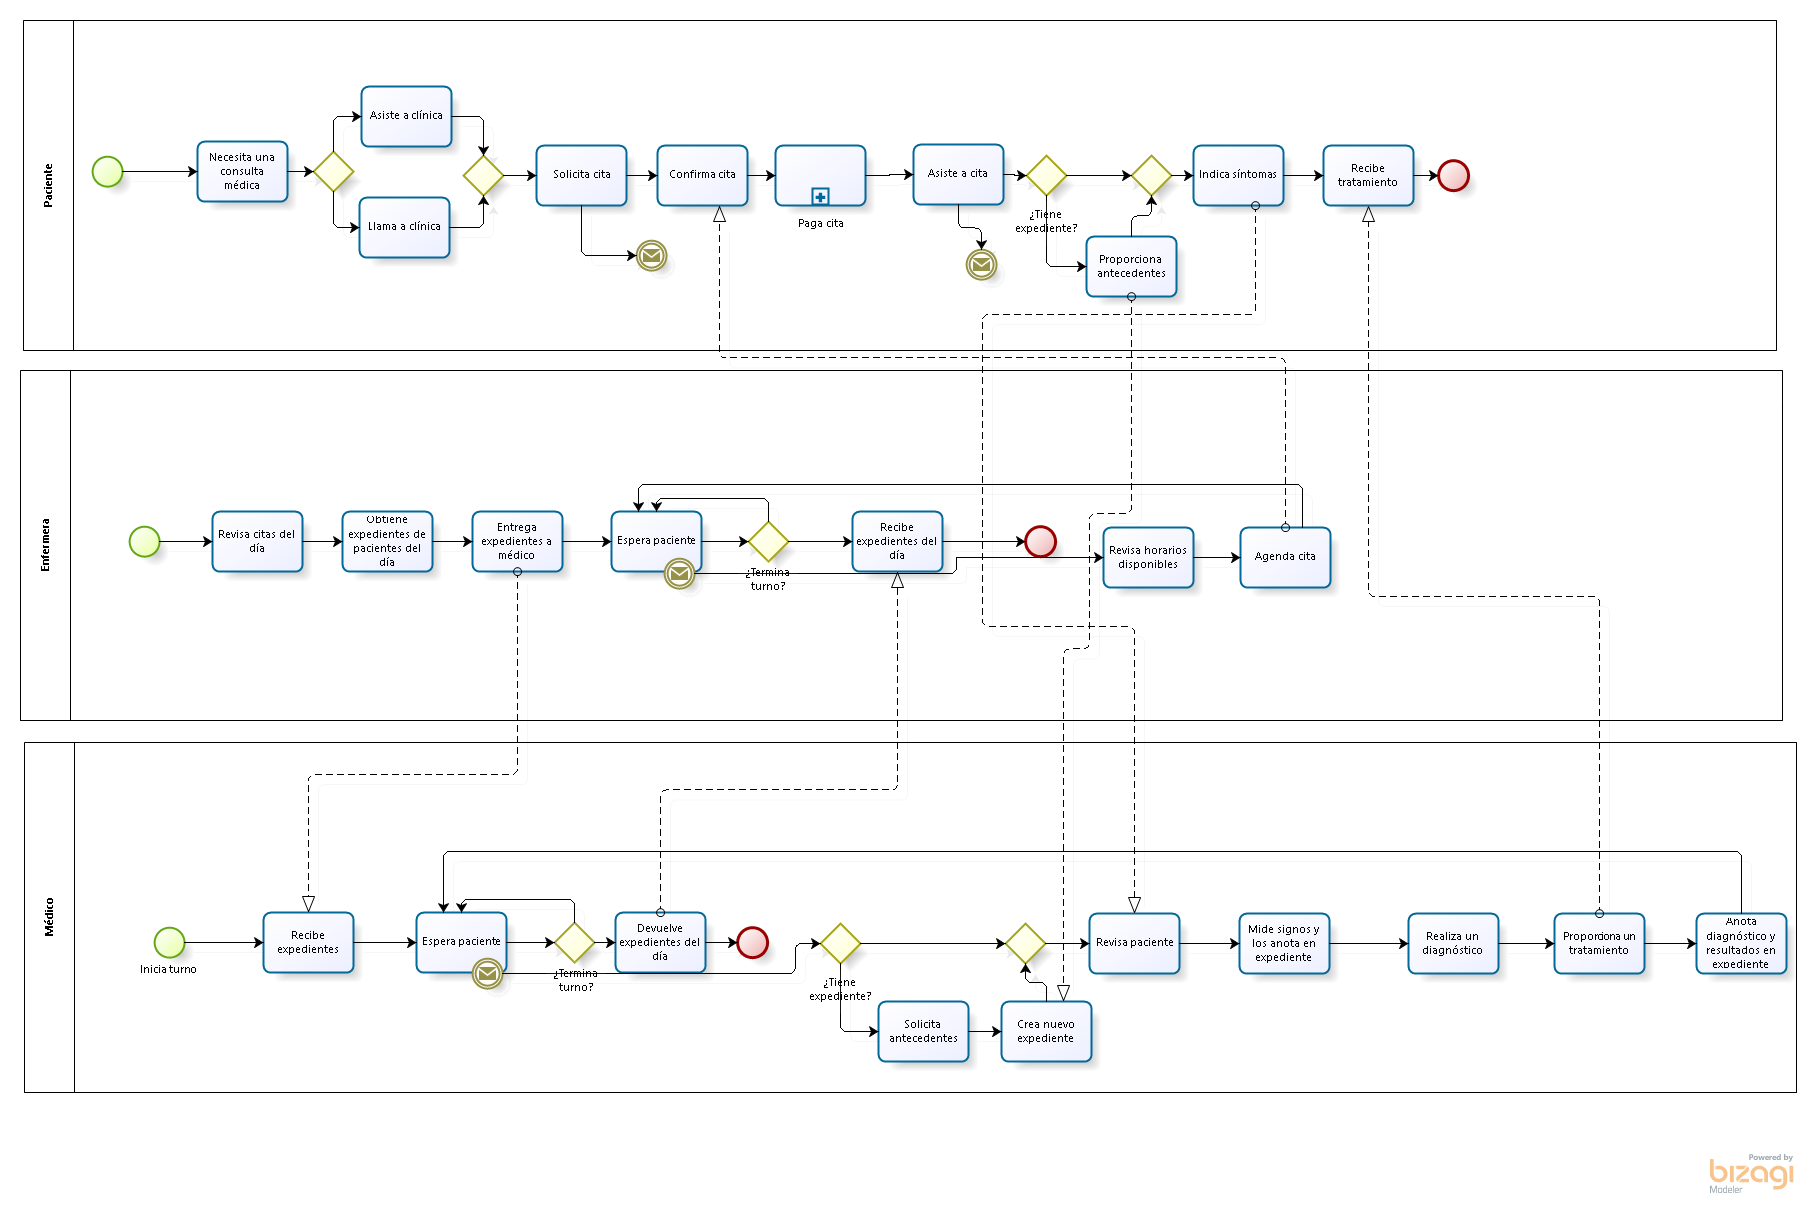
\includegraphics[width=1\textwidth]{images/Proceso_actual_citas}
		\caption{Diagrama del proceso actual citas.}
	\end{figure}
    \newpage
    \subsection{Proceso de pago de citas}

\begin{figure}[htbp!]
		\centering
			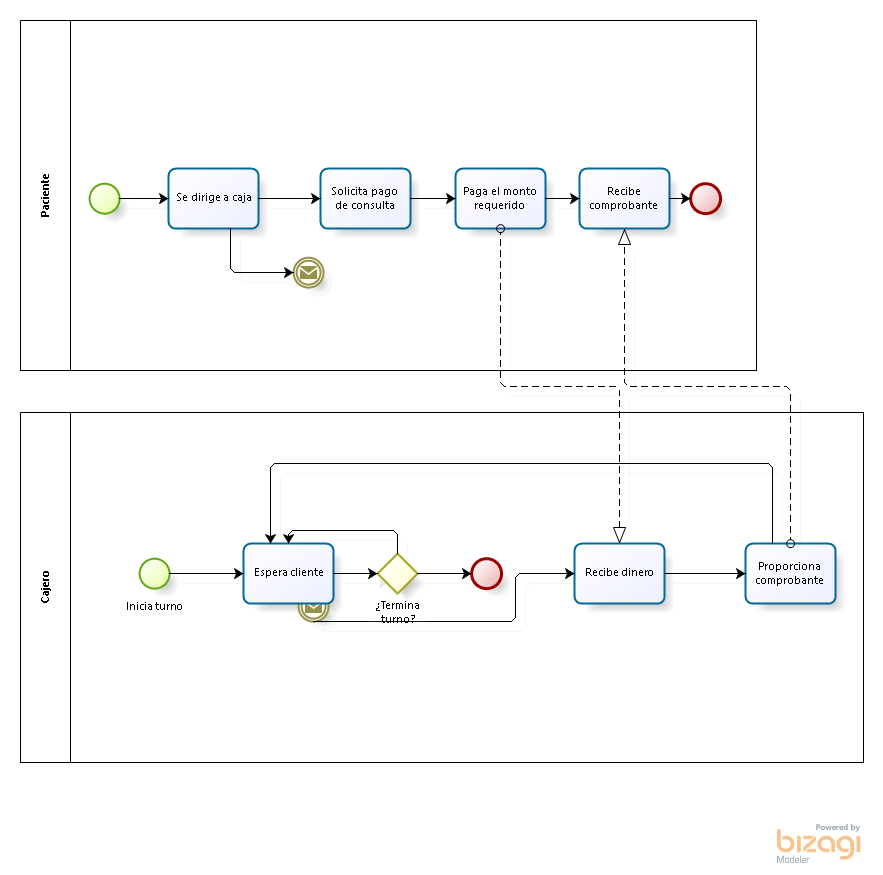
\includegraphics[width=0.5\textwidth]{images/Proceso_actual_pago_citas}
		\caption{Diagrama del proceso actual de pago de citas.}
	\end{figure}

\subsection{Proceso de adquisición de medicamentos}

\begin{figure}[htbp!]
		\centering
			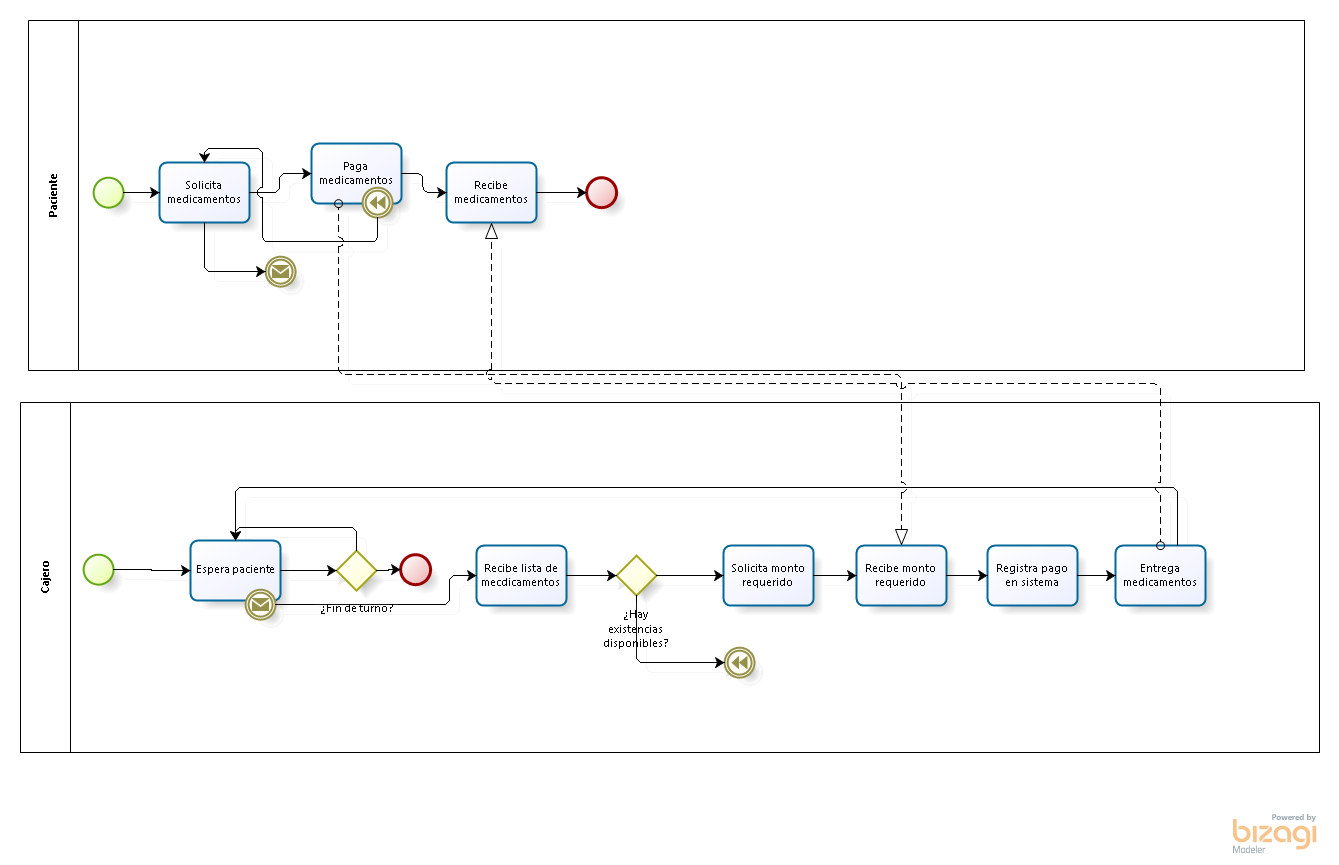
\includegraphics[width=0.7\textwidth]{images/Proceso_actual_medicamentos}
		\caption{Diagrama del proceso actual de adquisición de medicamentos.}
	\end{figure}
    \newpage
